\documentclass[10pt]{article}

% Pacotes extras necessários
\usepackage{amsmath}
\usepackage[lmargin=0.5in, rmargin=0.5in, tmargin=0.5in, bmargin=0.5in, includehead, includefoot]{geometry}
\usepackage{amsfonts}
\usepackage[utf8]{inputenc}
\usepackage[portuguese]{babel}
\usepackage{graphicx}
\usepackage{fancyhdr}
\usepackage{setspace}
\usepackage{listings}
\usepackage{url}
\usepackage{enumitem}

% More defined colors
\usepackage[dvipsnames]{xcolor}
 
% Required package
\usepackage{tikz}
\usetikzlibrary{positioning}

\graphicspath{ {./images/} }

% Sets para outras partes
\setlength{\parindent}{0pt}
\setstretch{1.5}
\DeclareMathOperator{\sen}{sen}
\DeclareMathOperator{\sinc}{sinc}

%% Facilidades
%% -- Laplace
\newcommand{\Lap}[1]{\mathcal{L}\left\{#1\right\}}

%% -- Negrito em matemáticas
\newcommand{\bm}[1]{\boldsymbol{#1}}


% ------- Estilo do trabalho -------- %
\fancypagestyle{capa}{
    \fancyhf{}
    \renewcommand\headrulewidth{0pt}
}

\pagestyle{fancy}
\fancyhead{}
\fancyhead[L]{\thepage}
\fancyfoot{}
% ----------------------------------- %

% Dados do Grupo
\title{Modelagem de Sistemas Dinâmicos - Trabalho Nº3}
\author{
    Leonardo Soares da Costa Tanaka - DRE: 121067652 \\
    Engenharia de Controle e Automação/UFRJ \\
    Rio de Janeiro, Brasil \\
    Julho de 2023
}
\date{}

\begin{document}
\maketitle
\thispagestyle{capa}

\quad Considerando um sistema de pêndulo invertido montado numa plataforma de 2 rodas:

\begin{figure}[h]
    \centering
    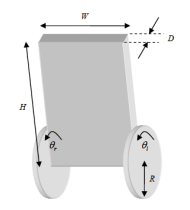
\includegraphics[scale=1.2]{fig1.png}
\end{figure}

\quad A vista lateral e superior deste sistema com as variáveis associadas é mostrada na seguinte
figura:

\begin{figure}[h]
    \centering
    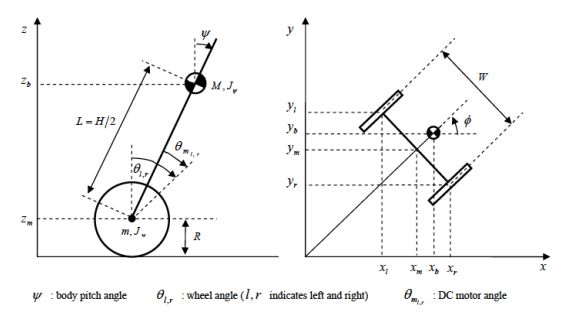
\includegraphics[scale=1.2]{fig2.png}
\end{figure}

\quad Os parâmetros físicos deste sistema são dados por:

\begin{itemize}
    \item $g = 9.8 \text{m/s}^2$: gravidade
    \item $m = 0.03 \text{kg}$: peso da roda
    \item $R = 0.04 \text{m}$: raio da roda
    \item $J_W = \frac{m R^2}{2}$: momento de inércia da roda
    \item $M = 0.6 \text{kg}$: peso do corpo
    \item $W = 0.14 \text{m}$: largura do corpo
    \item $D = 0.04 \text{m}$: profundidade do corpo
    \item $H = 0.144 \text{m}$: altura do corpo
    \item $L = \frac{H}{2}$: distância do centro de massa do corpo ao eixo da roda
    \item $J_{\psi} = \frac{ML^2}{3} \text{kgm}^2$: momento de inércia do corpo em pitch
    \item $J_{\phi} = \frac{M(W^2 + D^2)}{12} \text{kgm}^2$: momento de inércia do corpo em rumo
    \item $J_m$: inércia do motor DC desprezível
    \item $R_m = 6.69 \Omega$: resistência do motor DC
    \item $L_m$: indutância do motor desprezível
    \item $K_t = Ke = 0.4$: constante de torque (Nm/A) e constante de EMF (V s/rad)
    \item $f_m = 0.0022$: atrito entre o corpo e o motor
    \item $n = 1$: redução do motor
\end{itemize}

\quad Considerando os graus de liberdade $\{\theta, \psi, \phi \}$ onde $\theta = (\theta_l + \theta_r)/2 \rightarrow \dot{\theta} = (\dot{\theta_l} + \dot{\theta_r})/2$.

\quad A posição cartesiana do carrinho (composto pelas 2 rodas), no sistema de coordenadas
$\{x, y, x\}$, é dada por:

\begin{equation}
    X_m =
    \begin{bmatrix}
        x_m \\
        y_m \\
        z_m
    \end{bmatrix} =
    \begin{bmatrix}
        x_m \\
        y_m \\
        R
    \end{bmatrix}
\end{equation}

\quad Considerando que as rodas do carrinho não escorregam,
o carrinho é um sistema com restrições não-holonômicas,
sendo que a velocidade do carrinho é dada por:

\begin{equation}
    \dot{X_m} = R
    \begin{bmatrix}
        cos(\phi) \\
        sin(\phi) \\
        0
    \end{bmatrix}
    \dot{\theta}
\end{equation}

\quad A posição cartesiana das rodas (esquerda e direita) no sistema de coordenadas $\{x, y, x\}$,
é dada por:

\begin{equation}
\begin{aligned}
    X_l =
    \begin{bmatrix}
        x_l \\
        y_l \\
        z_l
    \end{bmatrix} =
    X_m + \frac{W}{2}
    \begin{bmatrix}
        - sin(\phi) \\
        cos(\phi) \\
        0
    \end{bmatrix}  \\
    X_r =
    \begin{bmatrix}
        x_r \\
        y_r \\
        z_r
    \end{bmatrix} =
    X_m + \frac{W}{2}
    \begin{bmatrix}
        sin(\phi) \\
        - cos(\phi) \\
        0
    \end{bmatrix}
\end{aligned}
\end{equation}

\quad A velocidade cartesiana das rodas é dada por:

\begin{equation}
    \begin{aligned}
        \dot{X_l} =
        \dot{X_m} + \frac{W}{2}
        \begin{bmatrix}
            - cos(\phi) \\
            - sin(\phi) \\
            0
        \end{bmatrix} \dot{\phi} \\
        \dot{X_r} =
        \dot{X_m} + \frac{W}{2}
        \begin{bmatrix}
            cos(\phi) \\
            sin(\phi) \\
            0
        \end{bmatrix} \dot{\phi}
    \end{aligned}
\end{equation}

\quad A posição cartesiana do corpo no sistema de coordenadas $\{x, y, x\}$,
é dada por:

\begin{equation}
    X_b = 
    \begin{bmatrix}
        x_b \\
        y_b \\
        z_b
    \end{bmatrix} = X_m + L
    \begin{bmatrix}
        cos(\phi) sin(\psi) \\
        sin(\phi) sin(\psi) \\
        cos(\psi)
    \end{bmatrix}
\end{equation}

\quad A velocidade cartesiana do corpo é dada por:

\begin{equation}
    \dot{X_b} = \dot{X_m} + L
    \begin{bmatrix}
        cos(\phi) cos(\psi) \\
        sin(\phi) cos(\psi) \\
        -sin(\psi)
    \end{bmatrix} \dot{\psi} + L
    \begin{bmatrix}
        -sin(\phi) sin(\psi) \\
        cos(\phi) sin(\psi) \\
        0
    \end{bmatrix} \dot{\phi}
\end{equation}

\quad Levando em consideração que a massa do motor DC é desprezível e
utilizando a fórmula de energia cinética translacional de um único corpo,
a energia cinética translacional é dada por:

\begin{equation}
    K_{tra} = \frac{1}{2} m \|\vec{v}\|^2
\end{equation}

\begin{equation}
\begin{gathered}
    T_1 = \frac{1}{2}m \dot{X_l^T} \dot{X_l} +
    \frac{1}{2}m \dot{X_r^T} \dot{X_r} +
    \frac{1}{2}M \dot{X_b^T} \dot{X_b} = \\
    = \frac{1}{2}m
    \begin{bmatrix}
        R cos(\phi) \dot{\theta} - \frac{W}{2}cos(\phi)\dot{\phi}
        & R sin(\phi) \dot{\theta} - \frac{W}{2}sin(\phi)\dot{\phi}
        & 0
    \end{bmatrix}
    \begin{bmatrix}
        R cos(\phi) \dot{\theta} - \frac{W}{2}cos(\phi)\dot{\phi} \\
        R sin(\phi) \dot{\theta} - \frac{W}{2}sin(\phi)\dot{\phi} \\
        0
    \end{bmatrix} + \\
    \frac{1}{2}m
    \begin{bmatrix}
        R cos(\phi) \dot{\theta} + \frac{W}{2}cos(\phi)\dot{\phi}
        & R sin(\phi) \dot{\theta} + \frac{W}{2}sin(\phi)\dot{\phi}
        & 0
    \end{bmatrix}
    \begin{bmatrix}
        R cos(\phi) \dot{\theta} + \frac{W}{2}cos(\phi)\dot{\phi} \\
        R sin(\phi) \dot{\theta} + \frac{W}{2}sin(\phi)\dot{\phi} \\
        0
    \end{bmatrix} + \\
    \scalebox{0.7}{$
    \frac{1}{2}M
    \begin{bmatrix}
        R cos(\phi) \dot{\theta} + L cos(\phi)cos(\psi)\dot{\psi} - L sin(\phi)sin(\psi)\dot{\phi}
        & R sin(\phi) \dot{\theta} + L sin(\phi)cos(\psi)\dot{\psi} + L cos(\phi)sin(\psi)\dot{\phi}
        & -L sin(\psi) \dot{\psi}
    \end{bmatrix}
    \begin{bmatrix}
        R cos(\phi) \dot{\theta} + L cos(\phi)cos(\psi)\dot{\psi} - L sin(\phi)sin(\psi)\dot{\phi}
        \\ R sin(\phi) \dot{\theta} + L sin(\phi)cos(\psi)\dot{\psi} + L cos(\phi)sin(\psi)\dot{\phi}
        \\ -L sin(\psi) \dot{\psi}
    \end{bmatrix} =
    $} \\
    = \frac{1}{2}m \left[R^2cos(\phi)^2\dot{\theta}^2 - WR cos(\phi)^2\dot{\theta}\dot{\phi} + \frac{W^2}{4}cos(\phi)\dot{\phi}^2 + R^2sin(\phi)^2\dot{\theta}^2 - WR sin(\phi)^2\dot{\theta}\dot{\phi} + \frac{W^2}{4}sin(\phi)\dot{\phi}^2\right] + \\
    \frac{1}{2}m \left[R^2cos(\phi)^2\dot{\theta}^2 + WR cos(\phi)^2\dot{\theta}\dot{\phi} + \frac{W^2}{4}cos(\phi)\dot{\phi}^2 + R^2sin(\phi)^2\dot{\theta}^2 + WR sin(\phi)^2\dot{\theta}\dot{\phi} + \frac{W^2}{4}sin(\phi)\dot{\phi}^2\right] + \\
    \scalebox{0.7}{$
    \frac{1}{2}M \left[ R^2cos(\phi)^2\dot{\theta}^2 + L^2cos(\phi)^2cos(\psi)^2\dot{\psi}^2 + L^2sin(\phi)^2sin(\psi)^2\dot{\phi}^2 + 2RLcos(\phi)^2cos(\psi)\dot{\theta}\dot{\psi} - 2L^2sin(\phi)cos(\phi)sin(\psi)\dot{\phi}\dot{\psi} - 2RLsin(\phi)cos(\phi)sin(\psi)\dot{\theta}\dot{\phi} \right] +
    $}\\
    \scalebox{0.7}{$
    \frac{1}{2}M \left[ R^2sin(\phi)^2\dot{\theta}^2 + L^2sin(\phi)^2cos(\psi)^2\dot{\psi}^2 + L^2cos(\phi)^2sin(\psi)^2\dot{\phi}^2 + 2RLsin(\phi)^2cos(\psi)\dot{\theta}\dot{\psi} + 2L^2sin(\phi)cos(\phi)sin(\psi)\dot{\phi}\dot{\psi} + 2RLsin(\phi)cos(\phi)sin(\psi)\dot{\theta}\dot{\phi} \right] +
    $}\\
    \frac{1}{2}M = L^2sin(\psi)^2\dot{\psi}^2 = \\
    \scalebox{1.1}{$
    = \frac{m \left[R^2\dot{\theta}^2 - WR\dot{\theta}\dot{\phi} + \frac{W^2}{4}\dot{\phi}^2 + R^2\dot{\theta}^2 + WR\dot{\theta}\dot{\phi} + \frac{W^2}{4}\dot{\phi}^2\right] + M \left[ R^2 \dot{\theta}^2 + L^2cos(\psi)^2\dot{\psi}^2 + L^2 sin(\psi)^2 \dot{\phi}^2 + 2RL cos(\psi)\dot{\theta}\dot{\psi} + L^2sin(\psi)^2\dot{\psi}^2 \right]}{2} =
    $}\\
    = \frac{m \left[2R^2\dot{\theta}^2 + \frac{W^2}{2}\dot{\phi}^2\right] + M \left[ R^2 \dot{\theta}^2 + L^2\dot{\psi}^2 + L^2 sin(\psi)^2 \dot{\phi}^2 + 2RL cos(\psi)\dot{\theta}\dot{\psi}\right]}{2}
\end{gathered}
\end{equation}

\quad Utilizando a fórmula da energia cinética rotacional:

\begin{equation}
\begin{gathered}
    K_{rot} = \frac{1}{2} \vec{\omega} \cdot \mathbf{I} \cdot \vec{\omega} \\
    T_2 = \frac{J_{\phi}\dot{\phi}^2}{2} + \frac{J_{\psi}\dot{\psi}^2}{2} + \frac{J_w(\dot{\theta}_r^2 + \dot{\theta}_l^2)}{2} + \frac{J_m n^2(\dot{\theta}_l - \dot{\psi})^2}{2} + \frac{J_m n^2(\dot{\theta}_r - \dot{\psi})^2}{2}
\end{gathered}
\end{equation}

\quad Considerando que $\dot{\theta} = (\dot{\theta}_l + \dot{\theta}_r)/2$, temos que:

\begin{equation}
\begin{gathered}
    \dot{\theta}_r^2 + \dot{\theta}_l^2 = 2\dot\theta^2 + \frac{W^2}{2R^2}\dot\phi^2, \quad (\dot{\theta}_l - \dot{\psi})^2 + (\dot{\theta}_r - \dot{\psi})^2 = 2(\dot\theta -\dot\psi)^2 + \frac{W^2}{2R^2}\dot\phi^2 \\
    \dot\phi =\frac{R}{W}\left(\dot\theta_r - \dot\theta_l\right)
\end{gathered}
\end{equation}

\quad Levando em consideração que $J_m$ é desprezível e utilizando as fórmulas acima, então:

\begin{equation}
\begin{gathered}
    T_2 = J_w \dot{\theta}^2 + \frac{1}{2} J_{\psi} \dot{\psi}^2 + \frac{1}{2} \left( J_{\phi} + \frac{W^2}{2R^2} J_w + \frac{W^2}{2R^2} n^2 J_m \right) \dot{\phi}^2 + n^2 J_m (\dot{\theta} - \dot{\psi})^2 \\
    T_2 = J_w \dot{\theta}^2 + \frac{1}{2} J_{\psi} \dot{\psi}^2 + \frac{1}{2} \left( J_{\phi} + \frac{W^2}{2R^2} J_w \right) \dot{\phi}^2
\end{gathered}
\end{equation}

\quad A energia potencial do sistema pode ser descrito pela soma das energias potenciais dos centros de massa das rodas e do corpo, tal que:

\begin{equation}
    U = mgz_l + mgz_r + mgz_b = 2mgR + Mg(R + Lcos(\psi))
\end{equation}

\section{Derivação e obtenção das equações dinâmicas}

\quad Levando em consideração que o Lagrangiano do sistema pode ser descrito pela seguinte equação e os valores de $T_1$, $T_2$ e $U$:

\begin{equation}
\begin{gathered}
    L = T_1 + T_2 - U  \\
    \scalebox{0.9}{$
    L = \frac{m \left[2R^2\dot{\theta}^2 + \frac{W^2}{2}\dot{\phi}^2\right] + M \left[ R^2 \dot{\theta}^2 + L^2\dot{\psi}^2 + L^2 sin(\psi)^2 \dot{\phi}^2 + 2RL cos(\psi)\dot{\theta}\dot{\psi}\right]}{2}
    + J_w \dot{\theta}^2 + \frac{1}{2} J_{\psi} \dot{\psi}^2 + \frac{1}{2} \left( J_{\phi} + \frac{W^2}{2R^2} J_w \right) \dot{\phi}^2
    - 2mgR - Mg(R + Lcos(\psi))
    $}
\end{gathered}
\end{equation}

\quad Temos que:

\begin{equation}
\begin{gathered}
    \frac{\partial L}{ \partial \theta} = 0, \ \frac{\partial L}{ \partial \psi} = ML^2sin(\psi)cos(\psi)\dot{\phi}^2 - MRLsin(\psi)\dot{\theta}\dot{\psi} + MgLsin(\psi), \ \frac{\partial L}{ \partial \phi} = 0 \\
    \frac{\partial L}{ \partial \dot{\theta}} = 2mR^2\dot{\theta} + MR^2\dot{\theta} + 2J_w\dot{\theta} + MRLcos(\psi)\dot{\theta} \\
    \frac{d}{dt} \left(\frac{\partial L}{ \partial \dot{\theta}}\right) = 2mR^2\ddot{\theta} + MR^2\ddot{\theta} + 2J_w\ddot{\theta} - MRLsin(\psi)\dot{\psi}^2 + MRLcos(\psi)\ddot{\psi} \\
    \frac{\partial L}{ \partial \dot{\psi}} = ML^2\dot{\psi} + MRLcos(\psi)\dot{\theta} + j_\psi \dot{\psi} \\
    \frac{d}{dt} \left(\frac{\partial L}{ \partial \dot{\psi}}\right) = ML^2\ddot{\psi} + j_\psi \ddot{\psi} - MRLsin(\psi)\dot{\theta}\dot{\psi} + MRLcos(\psi)\ddot{\theta} \\
    \frac{\partial L}{ \partial \dot{\phi}} = m\frac{W^2}{2}\dot{\phi} + ML^2sin(\psi)^2\dot{\phi} + \left( J_{\phi} + \frac{W^2}{2R^2} J_w \right) \dot{\phi} \\
    \frac{d}{dt} \left(\frac{\partial L}{ \partial \dot{\phi}}\right) = m\frac{W^2}{2}\ddot{\phi} + ML^2sin(\psi)^2\ddot{\phi} + 2ML^2sin(\psi)cos(\psi)\dot\psi\dot\phi + \left( J_{\phi} + \frac{W^2}{2R^2} J_w \right) \ddot{\phi}
\end{gathered}
\end{equation}

\quad (a) Utilizando a formulação de Lagrange foi determinado a dinâmica entre as coordenadas generalizadas $\lambda = \begin{bmatrix} \theta & \psi & \phi \end{bmatrix}^T$ e
as forças (torques) generalizadas $F = \begin{bmatrix} F_{\theta} & F_{\psi} & F_{\phi} \end{bmatrix}^T$.

\begin{equation}
    \frac{d}{dt}\left(\frac{\partial L}{\partial \dot{\lambda}}\right) - \frac{\partial L}{\partial \lambda} = F
\end{equation}

\quad Utilizando a fórmula acima e outras equações (14) para começar a montar a forma matricial:

\begin{equation}
\begin{gathered}
    \left[(2m + M)R^2 + J_w\right] \ddot{\theta} + MRLcos(\psi)\ddot{\psi} - MRLsin(\psi)\dot{\psi}^2 = F_{\theta} \\
    MRLcos(\psi)\ddot{\theta} + (ML^2 + J_\psi)\ddot{\psi} - ML^2sin(\psi)cos(\psi)\dot{\phi}^2 - MgLsin(\psi) = F_{\psi} \\
    \left[m\frac{W^2}{2} + ML^2sin(\psi)^2 + J_{\phi} + \frac{W^2}{2R^2} J_w \right]\ddot{\phi} + 2ML^2sin(\psi)cos(\psi)\dot{\psi}\dot{\phi} = F_{\phi}
\end{gathered}
\end{equation}

\quad Esta dinâmica pode ser escrita em forma matricial como:
\begin{equation}
    M(\lambda) \ddot{\lambda} + C(\lambda, \dot{\lambda}) + G(\lambda) = F
\end{equation}
onde $M(\cdot) \in \mathbb{R}^{3 \times 3}, \ C(\cdot, \cdot) \in \mathbb{R}^3, \ G(\cdot) \in \mathbb{R}^3$.

\quad Utilizando as equações (16) em forma matricial:

\begin{equation}
    \scalebox{0.85}{$
    \begin{bmatrix}
        (2m + M)R^2 + 2J_w & MRLcos(\psi) & 0 \\
        MRLcos(\psi) & ML^2 + J_\psi & 0 \\
        0 & 0 & M\frac{W^2}{2}+ML^2sin(\psi)^2+J_{\phi}+\frac{W^2}{2R^2}J_w
    \end{bmatrix} \ddot{\lambda}+
    \begin{bmatrix}
        - MRLsin(\psi)\dot{\psi}^2 \\
        - ML^2sin(\psi)cos(\psi)\dot{\psi}^2 \\
        2ML^2sin(\psi)cos(\psi)\dot\psi\dot\phi
    \end{bmatrix} +
    \begin{bmatrix}
        0 \\
        - MgLsin(\psi) \\
        0
    \end{bmatrix} = F
    $}
\end{equation}

\quad (b) Determinando a relação entre as forças generalizadas e os torques de
cada um das rodas $\{Fl,Fr\}$:

\begin{equation}
    F =
    \begin{bmatrix}
        F_{\theta} \\
        F_{\psi} \\
        F_{\phi}
    \end{bmatrix} = E
    \begin{bmatrix}
        F_l \\
        F_r
    \end{bmatrix}
\end{equation}

onde $E \in \mathbb{R}^{3\times 2}$

\quad Observando o sistema de pêndulo invertido e os graus de liberdade,
é possível determinar as seguintes relações:

\begin{equation}
\begin{gathered}
    F_\theta = F_l + F_r \\
    F_\psi = - F_l - F_r \\
    F_\phi = - \frac{W}{2R}F_l + \frac{W}{2R}F_r \\
    F =
    \begin{bmatrix}
        F_{\theta} \\
        F_{\psi} \\
        F_{\phi}
    \end{bmatrix} =
    \begin{bmatrix}
        1 & 1 \\
        -1 & -1 \\
        -\frac{W}{2R} & \frac{W}{2R}
    \end{bmatrix}
    \begin{bmatrix}
        F_l \\
        F_r
    \end{bmatrix} 
\end{gathered}
\end{equation}

\quad (c) Determinando a relação entre as forças (torques) generalizadas $\{F_\theta, F_\psi, F_\phi\}$
e a tensão elétrica aplicada em cada motor $\{Vl,Vr\}$ utilizando o modelo de um motor DC:

\begin{equation}
    F = Q \dot\lambda + H
    \begin{bmatrix}
        V_l \\ V_r
    \end{bmatrix}
\end{equation}

onde $Q \in \mathbb{R}^{3 \times 3}$ e $H \in \mathbb{R}^{3 \times 2}$.

\quad Levando em consideração a Lei de Kirchhoff das Tensões, a Equação do Torque, a Lei do Motor e a Lei do Gerador.
Além disso, o atrito entre o corpo e o motor e o indutância do motor DC $L_m$ é desprezível:

\begin{equation}
\begin{gathered}
    F_{l,r} = nK_ti_{l,r} + f_m(\dot\psi - \dot\theta_{l,r}) \\
    V_{l,r} + K_e(\dot\psi - \dot\theta_{l,r}) = L_m\dot{i}_{l_r} + R_mi_{l,r} \\
    i_{l,r} = \frac{V_{l,r} + K_e(\dot\psi - \dot\theta_{l,r})}{R_m} \\
    F_{l,r} = \left(\frac{nK_tK_e}{R_m} + f_m\right)(\dot\psi - \dot\theta_{l,r}) + \frac{nK_tV_{l,r}}{R_m}
\end{gathered}
\end{equation}

\quad Pegando a relação (20) entre as forças generalizadas e os torques de
cada um das rodas $\{Fl,Fr\}$ e substituindo $\{Fl,Fr\}$ pelos valores obtidos (22):

\begin{equation}
\begin{gathered}
    F =
    \begin{bmatrix}
        1 & 1 \\
        -1 & -1 \\
        -\frac{W}{2R} & \frac{W}{2R}
    \end{bmatrix}
    \begin{bmatrix}
        F_l \\
        F_r
    \end{bmatrix} =
    \begin{bmatrix}
        1 & 1 \\
        -1 & -1 \\
        -\frac{W}{2R} & \frac{W}{2R}
    \end{bmatrix}
    \begin{bmatrix}
        \left(\frac{nK_tK_e}{R_m} + f_m\right)(\dot\psi - \dot\theta_l) + \frac{nK_tV_r}{R_m} \\
        \left(\frac{nK_tK_e}{R_m} + f_m\right)(\dot\psi - \dot\theta_r) + \frac{nK_tV_r}{R_m}
    \end{bmatrix} \\
    F =
    \begin{bmatrix}
        -2\left(\frac{nK_tK_e}{R_m} + f_m\right) & 2\left(\frac{nK_tK_e}{R_m} + f_m\right) & 0 \\
        2\left(\frac{nK_tK_e}{R_m} + f_m\right) & -2\left(\frac{nK_tK_e}{R_m} + f_m\right) & 0 \\
        0 & 0 & - \frac{W^2}{2R^2} \left(\frac{nK_tK_e}{R_m} + f_m\right)
    \end{bmatrix}
    \begin{bmatrix} \dot\theta \\ \dot\psi \\ \dot\phi \end{bmatrix}
    +
    \begin{bmatrix}
        \frac{nK_t}{R_m} & \frac{nK_t}{R_m} \\
        -\frac{nK_t}{R_m} & -\frac{nK_t}{R_m} \\
        -\frac{W}{2R}\frac{nK_t}{R_m} & \frac{W}{2R}\frac{nK_t}{R_m}
    \end{bmatrix}
    \begin{bmatrix}
        V_l \\ V_r
    \end{bmatrix}
\end{gathered}
\end{equation}

\section{Derivação e obtenção das equações de estado}

\quad Defininado as variáveis de estado do sistema:

\begin{equation}
    x_1 = \lambda =
    \begin{bmatrix}
        \theta \\
        \psi \\
        \phi
    \end{bmatrix}, \quad
    x_2 = \dot\lambda = 
    \begin{bmatrix}
        \dot\theta \\
        \dot\psi \\
        \dot\phi
    \end{bmatrix}
\end{equation}

\quad Derivando as variáveis de estado do sistema e utilizando as representação (24) como base:

\begin{equation}
    \dot{x_1} = \dot\lambda = x_2 =
    \begin{bmatrix}
        \dot\theta \\
        \dot\psi \\
        \dot\phi
    \end{bmatrix}
\end{equation}

\quad Para calcular o $M(\lambda)^{-1}$, será necessário calcular o determinante:

\begin{equation}
\begin{gathered}
    det(M) = 
    \begin{vmatrix}
        (2m + M)R^2 + 2J_w & MRLcos(\psi) & 0 \\
        MRLcos(\psi) & ML^2 + J_\psi & 0 \\
        0 & 0 & M\frac{MW^2}{2} + MLsin(\psi)^2 + J_\phi + \frac{W^2}{2R^2}J_w \\
    \end{vmatrix} = \\
    \scalebox{0.85}{$
    = [(2m + M)R^2 + 2J_w](ML^2 + J_\psi)(M\frac{MW^2}{2} + MLsin(\psi)^2 + J_\phi + \frac{W^2}{2R^2}J_w) -  M^2R^2L^2cos(\psi)^2(M\frac{MW^2}{2} + MLsin(\psi)^2 + J_\phi + \frac{W^2}{2R^2}J_w)
    $}
\end{gathered}
\end{equation}

\quad Além disso, é necessário calcular a matriz adjunta:

\begin{equation}
    \scalebox{0.65}{$
    M_{adj} =
    \begin{bmatrix}
        (ML^2 + J_\psi)(M\frac{W^2}{2}+ML^2sin(\psi)^2+J_{\phi}+\frac{W^2}{2R^2}J_w) & -MRLcos(\psi)(M\frac{W^2}{2}+ML^2sin(\psi)^2+J_{\phi}+\frac{W^2}{2R^2}J_w) & 0 \\
        -MRLcos(\psi)(M\frac{W^2}{2}+ML^2sin(\psi)^2+J_{\phi}+\frac{W^2}{2R^2}J_w) & [(2m + M)R^2 + 2J_w](M\frac{W^2}{2}+ML^2sin(\psi)^2+J_{\phi}+\frac{W^2}{2R^2}J_w) & 0 \\
        0 & 0 & [(2m + M)R^2 + 2J_w](ML^2 + J_\psi) - M^2R^2L^2cos(\psi)^2
    \end{bmatrix}
    $}
\end{equation}

\quad Utilizando o determinante e a matriz adjunta para encontrar $M(\lambda)^{-1}$:

\begin{equation}
    \scalebox{0.8}{$
    M(\lambda)^{-1} = \frac{M_{adj}}{det(M)} =
    \begin{bmatrix}
        \frac{ML^2 + J_\psi}{[(2m + M)R^2 + 2J_w](ML^2 + J_\psi) - M^2R^2L^2cos(\psi)^2} & -\frac{MRLcos(\psi)}{[(2m + M)R^2 + 2J_w](ML^2 + J_\psi) - M^2R^2L^2cos(\psi)^2} & 0 \\
        -\frac{MRLcos(\psi)}{[(2m + M)R^2 + 2J_w](ML^2 + J_\psi) - M^2R^2L^2cos(\psi)^2} & \frac{(2m + M)R^2 + 2J_w}{[(2m + M)R^2 + 2J_w](ML^2 + J_\psi) - M^2R^2L^2cos(\psi)^2} & 0 \\
        0 & 0 & \frac{1}{M\frac{MW^2}{2} + MLsin(\psi)^2 + J_\phi + \frac{W^2}{2R^2}J_w}
    \end{bmatrix}
    $}
\end{equation}

\quad Com isso, tenho tudo que é preciso para preencher a seguinte equação:

\begin{equation}
    \dot{x_2} = \ddot\lambda = M(\lambda)^{-1} \left( -C(\lambda,\dot\lambda) - G(\lambda) + F(\dot\lambda,V) \right)
\end{equation}

\end{document}